\section{Eine voreilige Pressekonferenz}

\begin{frame}{Der wissenschaftliche Durchbruch?}
    \pause
    \begin{columns}
        \begin{column}{0.6\textwidth}
            \begin{itemize}
                \item<+-> 1989: Pressekonferenz der Chemiker M.~Fleischmann und S.~Pons
                \item<+-> Behauptung Fusionsprozess im Reagenzglas bei Zimmertemperatur gefunden zu haben
                \item<+-> sehr große Resonanz bei der Presse
                \item<+-> Angeblich sollten während der Elektrolyse von $\mathrm{D_2O}$ die $\mathrm{D}$-Atome auf einer Palladiumkathode fusionieren
                \item<+-> Massive Kritik anderer Wissenschaftler am Stil der Veröffentlichung und Mängeln in der Arbeit
                \item<+-> die Ergebnisse konnten nicht bestätigt werden (auch nicht von Fleischmann und Pons selbst)
                \item<+-> bis heute gibt es mehr oder weniger seriöse Forschung an ähnlichen Versuchsaufbauten
            \end{itemize}
        \end{column}
        \begin{column}{0.4\textwidth}
            \begin{center}
                \only<2->{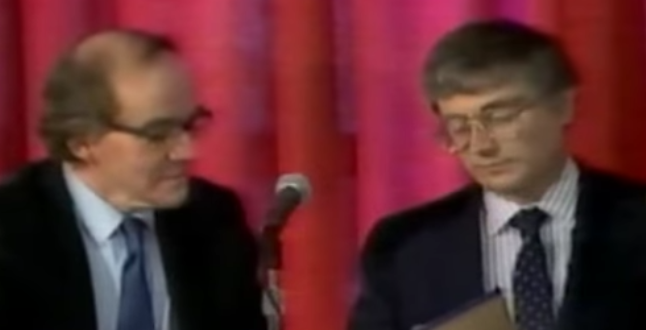
\includegraphics[width=0.8\textwidth]{images/FleischmannPons.png}
                \small{Fleischmann und Pons \cite{Pressekonferenz}}}
                
                \only<5->{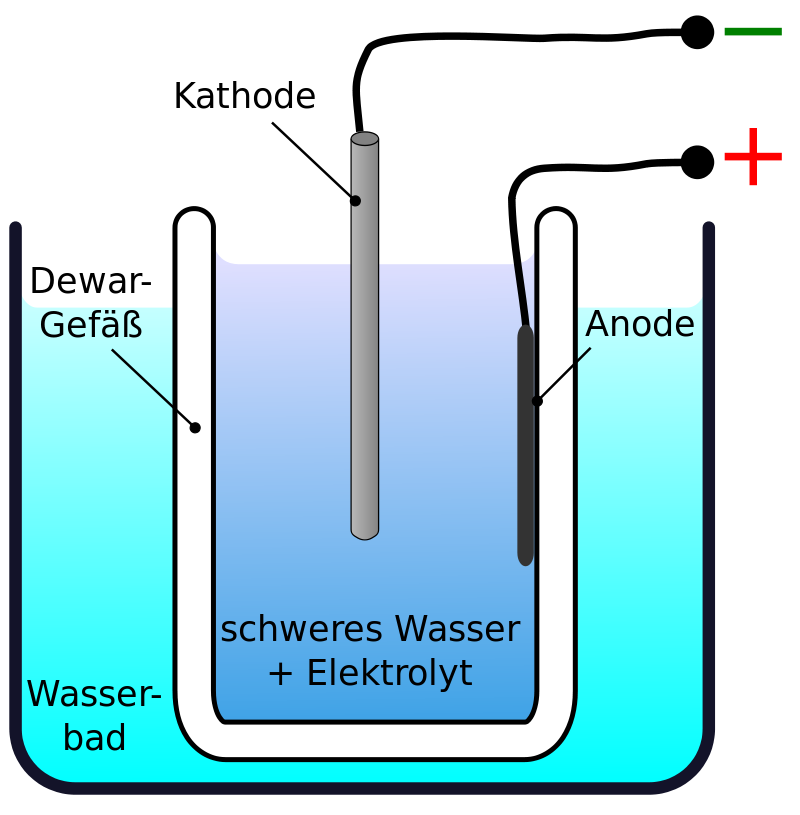
\includegraphics[width=0.7\textwidth]{images/FleischmannPonsAufbau.png}
                \small{Versuchsaufbau \cite{AufbauKalt}}}
            \end{center}
        \end{column}
    \end{columns}
\end{frame}
